\chapter{Вычислительные алгоритмы для задач моделирования биомеханики живых систем}\label{ch:ch1}

\section{Проблемы моделирование биомеханики сложных систем. Движение жидкости в эластичных капиллярах}\label{sec:ch1/sec1}

Новые методы, разрабатываемые математиками, физиками и программистами в сотрудничестве с биологами, позволяют создавать компьютерные модели сложных живых систем, которые могут адекватно воспроизводить свойства таких систем. В основе этих стремлений лежит интерес учёных к пониманию биологических и физических принципов функционирования живых организмов и их подсистем. В частности, наблюдается растущий интерес к исследованиям функций живого нейрона и целых нервных систем животных с использованием теории математического моделирования и новейших вычислительных систем, симулирующих нейронные контуры. Подробные математические модели, учитывающие базовые принципы распространения, обработки и хранения информации в нейронных контурах будут чрезвычайно востребованы для дальнейших исследований не только в области биологии и медицины, но и в области создания искусственного интеллекта.
Все это становится возможным благодаря появлению новых инструментов исследования биологических свойств клеток. Например, компьютерная технология восстановления схемы участка мозга из множества микрофотографий срезов нервной ткани \cite{CHKLOVSKII2010667} в трехмерной компьютерной модели, повторяющей точное морфологическое строение оцифрованного участка. В тоже время, совершенно очевидно, что без развития суперкомпьютеров, создания новых систем обработки больших массивов данных на на основе распределенных вычислений, а также  создания новых программных протоколов и языков программирования  появление таких методов вряд ли было бы возможно. Зачастую разработка компьютерных имитационных моделей биологических систем связана с обработкой, интерпретацией и анализом большого количества неоднородных данных. Однако, чем точнее модель, тем больше физических и физиологических особенностей необходимо учитывать.

В связи с несомненной актуальностью решения поставленной задачи в настоящее время по данной тематике реализуется целый ряд широкомасштабных международных проектов. Одним из них является проект «Human Brain Project» \cite{Markram2011}, являющийся логическим развитием проекта «Blue Brain Project» \cite{Markram2006}. Проект был запущен в 2013 году на базе Швейцарской высшей политехнической школы Лозанны. Основной целью является моделирование нейросети, включающей в себя порядка 100 млрд. нервных клеток и 100 трлн. синаптических связей. Можно предположить, что разработка такой модели будет основываться на методах, которые были созданы в течение работы над проектом «Blue Brain Project». За основу взята колонка неокортекса, включающая 10000 нейронов крысы, которая оцифрована и загружена в суперкомпьютер EPFL IBM Blue Gene/L, а затем многократно реплицирована на аналогичные компьютеры и объединена в единую сеть. Модель нейрона описывается при помощи программного пакета «NEURON» \cite{Carnevale2006} на специализированном интерпретируемом языке программирования HOC (high order calculation), ориентированного на создание моделей нейронов и сетей нейронов, основанных на экспериментальных данных. Одним из недостатков такого подхода является отсутствие описания структуры связей в нервной системе (коннектома мозга). «Механическое» копирование колонки мозга не позволяет создать полнофункциональную модель целого мозга. Помимо связей внутри колонки необходимо учитывать связи между колонками, как соседними, так и дальними, и другими отделами мозга, которые, весьма вероятно, для каждой колонки уникальны, не говоря уже о том, что неокортекс – лишь часть мозга.

В США, начиная с 2009 года, реализуется проект «Human Connectome Project» \cite{Elam2013}. Основной целью проекта на первом этапе является создание полного коннектома человеческого мозга. На финальной стадии предполагается создание электронной копии мозга человека, построенной на основе его коннектома. При этом оценить работоспособность модели можно будет лишь после того, как она будет полностью закончена и подключена к источникам внешней информации – зрительной, звуковой, тактильной и т.д. - в случае, если она окажется способной на коммуникацию. Проект носит протяженный характер и не имеет определенных сроков реализации.

В подобной ситуации, когда промежуточные итоги не позволяют судить о финальном результате проекта, крайне необходима разработка альтернативных подходов, которые могут реализовываться параллельно, имея более локальные цели, сжатые сроки реализации и менее сложный объект исследования. При этом весьма актуальной остается проблема проверки адекватности работы подобных систем, которая, по сути, невозможна без обеспечения работающей модели потоком входных сигналов, а ее исследователя – средствами анализа исходящих. Такая проверка представляется возможной, если выбрать в качестве объекта изучения достаточно простой многоклеточный организм, не ограничиваясь при моделировании обособленной нервной системой, а дополнив ее сенсорной и мышечной системами, образующими в совокупности с телом и мышцами организма самодостаточную нейроинформационную систему. Идеальным кандидатом для проведения исследований, связанных с полным моделированием нервной системы, по нашему мнению, является широко известный модельный организм - нематода \textit{C. elegans}. Строение нервной системы у всех особей одного пола практически идентично: 302 нейрона, около семи тысяч межнейронных соединений (~5000 тысяч соединений между собой и ~2000 – между нейронами и мышцами), 95 мышечных клеток, несколько десятков сенсорных клеток разного типа и примерно 86 соединений между нейронами и сенсорными клетками. Общее количество клеток, образующих тело нематоды также известно – 959. В настоящее время диаграмма связности нейронной сети C. elegans, по оценкам, определена приблизительно на 75-90%.

Несмотря на малый размер и жесткую детерминированность архитектуры нервной системы, характерную для простых организмов, C. elegans обладает достаточно широким набором поведенческих реакций и возможностей восприятия информации об окружающей среде, которое происходит посредством механо-, хемо- и терморецепторов; также обнаружено несколько нейронов, реагирующих на изменение освещённости. Нематода может обучаться: предпочитать участки пространства, сенсорные сигналы от которых на основе прежнего опыта позволяют прогнозировать наличие  пищи, и наоборот, избегать тех областей, которые могут быть связанными с негативными воздействиями. Также C. elegans обладает зачатками способностей к краткосрочной и долгосрочной памяти и проявляет ассоциативные формы обучения, такие как выработка классического и дифференцированного условного рефлекса. Эти свойства представляют особенный интерес, далеко выходящий за рамки выбранного модельного живого объекта, и являются фундаментальными для любой развитой нервной системы. Благодаря такой изученности \textit{C. elegans} ученые из многих лабораторий пытаются если не воспроизвести, то хотя бы приблизиться к реализации полной модели нематоды. В последние несколько десятилетий был создан ряд рабочих моделей, посвященных изучению различных аспектов биологии нематоды, ключевые работы и сравнение между ними представлены в таблице \ref{tab:test1}.

\begin{table} [htbp]% Пример записи таблицы с номером, но без отображаемого наименования
  \centering
  \begin{threeparttable}% выравнивание подписи по границам таблицы
    \caption{Сравнение различных моделей и подходов к симуляции C. elegans}%
    \label{tab:test1}%
    \begin{SingleSpace}
      \begin{tabular}{| c | c | c | c | c |}
        \hline
        Модель & \thead{Сложность,\\
            модель/окружение} & 2D/3D & Типы движения & Доступность \\ \hline
        \cite {NIEBUR19911132} & 40 частиц (19 сегментов)  & 2D  & Ползание & Нет данных  \\ \hline
        \cite {Bryden2004} & 11 сегментов  & 2D  & Ползанье & Нет данных  \\ \hline
        \cite {Suzuki2004} & {\makecell {13 жестких соединений, \\ 
        12 подвижных суставов}} & 2D  & Ползание & Нет данных \\ \hline
        \cite {Karbowski2008} & {\makecell {12 секций, \\ 
        локальные сгибаемые \\ 
        углы}} & 2D  & Ползание & {\makecell {ModelDB \\ 
        database}}
 \\ \hline
        \cite {Rnkk2008ModelingTC} & 39 частиц  & 3D  & Ползание & {\makecell {Закрытый \\ источник}}
 \\ \hline
    \cite {Mailler2010} & 100 частиц & 3D & Ползание & Нет данных \\ \hline
    \cite {Palyanov2012} & ~200 частиц & 3D & Ползание & {\makecell {Открытый 
    \\ исходный код}} \\ \hline
   \cite {Boyle2012} & 98 частиц & 2D & Ползание & {\makecell {Открытый 
   \\ исходный код}} \\ \hline
   \cite {Williamson2012} & {\makecell {25 жестких стержней, \\ 
   соединенных эластичными \\
   соединениями, \\
   представляющими \\
   мышцы тела}} & 2D & Ползание & {\makecell {Нет \\ 
   данных}} \\ \hline
   \cite {Palyanov2018} & {\makecell { 10143 \\
   эластичных частиц \\
   и 11436 \\
   частиц жидкости}} & 3D & {\makecell {Ползанье, \\
   Плаванье,\\
   Разворот\\
   Омега поворот}} & {\makecell {Открытый \\
   исходный код}} \\ \hline
      \end{tabular}%
    \end{SingleSpace}
  \end{threeparttable}
\end{table}

В большинстве описанных работ для моделирования тела нематоды часто использовались упрощенные механистические аналогии, представляющие тело в виде нескольких последовательных сегментов, зачастую линейных или более сложных форм, соединенных упругими суставами, способными сгибаться. Посредством этого, модель способна осуществлять волнообразное движение. Большинство моделей были сделаны на основе концепции массовых точек и пружин, где продольные упругие сегменты моделируют мышцы. Такое упрощение ограничивает модели только конкретным моделируемым поведением.

В тоже время разработанный в нашей лаборатории программный пакет \cite {Palyanov2016} для имитационного компьютерного моделирования, позволяет создавать гораздо более сложные и точные симуляции абстрагированные от конкретных задач, учитывающие большое количество физических параметров среды.

\section{Методы описания моделей движения биологических систем}\label{sec:ch1/sec2}


Одной из важнейших задач нейроинформатики является проблема исследования механизмов координации поведения нервной системой, решение которой без генерации входных и анализа выходных данных не представляется возможным. Как показано в работе \cite {Krichmar2005}, в качестве источника потока входных данных возможно использовать роботизированную систему, оснащенную сенсорами, действующую в реальном мире под управлением программного обеспечения, моделирующего нервную систему. Однако этот подход не всегда может быть применим так, например, в случае \textit{C. elegans}, маленькой нематоды 1 мм в длину, разработка подобного робота является трудновыполнимой задачей. Во-первых, на данный момент не существует возможности разработать робота в том же масштабе, что и живая нематода. Для \textit{C. elegans} масштаб играет важную роль, так как для того чтобы воспроизвести естественную среду обитания червя (почва в природе, агар в лабораторной чашке Петри), необходимо учитывать такие физические эффекты, как капиллярные силы, поверхностное натяжение, вязкость  и др. Во-вторых, другой серьезной сложностью при создании роботов являются временные и финансовые затраты на их разработку, что значительно усложняет работу с подобными моделями в территориально распределенных научно-исследовательских группах.

В нашей лаборатории был разработан программный пакет \cite {Palyanov2012} на базе которого была разработан, упрощенный трехмерный прототип - расширяемая интерактивная симуляция с трехмерным графическим интерфейсом, основной целью которой собрать все существующие и будущие данные описывающие биологические системы червя в виде функциональной интегрированной модели. Прототип – это трехмерная динамическая модель, которая включает в себя мышечную систему и часть нервной, взаимодействующие друг с другом в окружающем физическом пространстве. В ранних работах, посвященных исследованию движения \textit{C. elegans} и нервного контроля этого механизма, зачастую применялись только двумерные модели. В отличие от этих подходов мы создали динамическую, интерактивную трехмерную модель, в которой консолидировали,  симулировали и визуально представили данные об анатомии \textit{C. elegans}. Мышечная система \textit{C. elegans}, включает в себя 4 мышечных квадранта, проходящих по всей длине внутренней полости тела \cite {White1986}, что двумерная модель не смогла бы представить в полной мере. Как результат, в двумерной модели вводятся приближения на уровне соединений между моторными нейронами и мышцами, которые, в свою очередь, требуют компромиссов и аппроксимаций. Кроме того, визуализация нервной системы, привязанной к телу червя, дает возможность пользователю наблюдать зависимость между активностью моделируемой нервной системы и поведением.

Реализованная библиотека для симуляции физических законов реального мира, упрощает создание сложных динамических объектов, и предоставляет графический интерфейс для взаимодействия с пользователем. С помощью методов системного, объектно-ориенти­рованного программирования, была реализована архитектура приложения как композиция связанных абстрактных классов. Библиотека реализована на C++ с применением OpenGL для имплементации GUI (graphical user interface). Каждый объект может быть представлен как комбинация следующих примитивов: точечные массы, пружины (которые соединяют пару точечных масс), мышцы (активные пружины, которые сокращаются пропорционально интенсивности пришедшего на них сигнала от моторных нейронов), нейроны и соединения между нейронами или между нейронами и мышечными клетками. Для всех объектов были реализованы абстрактный классы инкапсулирующие свойства и методы характеризующие конкретный объект. Любая комбинация объектов, скомпонованная из примитивов, может быть собрана в более сложный объект в виртуальном физическом окружении. Между объектами могут быть определены связи. Один тип связи - это физический коннектор, который дает возможность одной точечной массе влиять на другие, связанные с ней пружинами или мышцами. Еще один вид связи - это физическое отталкивание, препятствующее проникновению сквозь объект, например взаимодействие точечных масс с плоскостью или поверхностью, такой как виртуальная «чашка Петри». Связи вместе с силами гравитации и трения определяют общую силу, действующую на каждую точечную массу в момент времени \( t \):
\[
F=\sum_{i} F_{i}^C + F^{external}
\]

Где \( F_{i}^C \) - силы взаимодействия объекта со связанными объектами, \( F^{external}  \)- сумма внешних сил. Вычислив общую силу, движение каждой точки в момент \( t + \Delta t \) рассчитывается при помощи численного интегрирования (шаг по времени \( \Delta t = 8 \cdot 10^{-3}c \)).

\begin{figure}[ht]
  \centerfloat{
    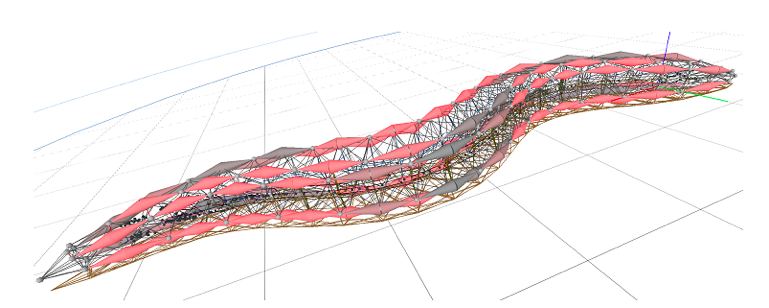
\includegraphics[scale=0.60]{cyber_elegans}
  }
  \caption{Интегрированная модель нематоды \textit{C. elegans.}}\label{fig:cyber_elegans}
\end{figure}

Несмотря на то, что довольно много биологических деталей опущено основная ценность данного прототипа заключается в доказательстве концепции того, что широкий ряд биофизических факторов - от сил, действующих на тело, до паттернов активации нейронов и движения мышц, может быть одновременно учтен и объединен в единую программную систему. На данный момент существуют более детализированные модели для двигательных систем \cite{Boyle2012} и лучшее представление для нейронов и нейросетей (NeuroML \cite {Gleeson2010} для мульти-сегментной модели) однако именно в нашей работе впервые была предложена концепция и продемонстрирован работающих прототип, объединяющий трехмерную модель тела с управляющим им фрагментом нейронной сети \cite {Palyanov2012}.

При моделирования физического тела биологического существа – от одной клетки до целого беспозвоночного организма – необходимо учитывать, каким образом в модели будут представлены механические свойства двух ее важнейших компонентов: упругого материала для внешней оболочки тела и жидкости, аппроксимирующей внутреннее содержимое тела. Части, ответственные за активное движение (такие как мышцы), также должны описываться как упругий материал, способный сокращаться под действием внешних стимулов. Жидкость также необходима для моделирования внешней среды. Трудно переоценить важность моделирования именно несжимаемой жидкости для реалистичного представления моделируемых объектов как с физической, так и с биологической точек зрения. И, наконец, необходима возможность описания и определения  взаимодействия между жидкостью и упругим материалом.

Учитывая все вышесказанное, все эти требования привели нас к тому, что в качестве базового метода моделирования механики сплошных сред был выбран метод частиц (Лагранжевый метод), как более подходящий для данной проблемы по сравнению с сеточными (Эйлеровыми) методами.  В свою очередь, это привело нас к использованию метода гидродинамики сглаженных частиц и его модификаций. Мы также представляем реализацию этого алгоритма, которая служат основой для моделирования тела нематоды \textit{C.elegans}. 3D модели как одиночной мышечной клетки, так и всего тела \textit{C.elegans} представлены в виде системы частиц и производится расчет их динамики для того, чтобы сравнить  механику мышечной клетки и модели тела с таковыми для реального организма.

Будущие результаты, полученные в этой области, могут дать новые знания о нейронных механизмах и паттернах, таких как, например, до сих пор неизвестный механизм, отвечающий за генерацию синусоидального паттерна движения. Эти результаты могут быть использованы в области дизайна искусственных нейронных сетей. Изучение возможности детальной репродукции нервной сети \textit{C. elegans} может стать  первым шагом в изучении более сложных нервных систем путем их компьютерного моделирования. Хотя часто говорят, что нервная система \textit{C. elegans} почти полностью исследована, предполагают только топологию и схему соединений между нейронами; в тоже время на более глубоких уровнях, таких как механизм преобразования сигнала и тип задействованных нейромедиаторов, нейросеть \textit{C. elegans} остается во многом неизученной.

Планируется встроить в симулятор реалистичные модели сокращения мышц \cite {Huxley1957MuscleSA}, моделирования нейронов \cite {Gleeson2010}, обеспечить работу механизмов, имитирующих сигналы, поступающие от сенсорных клеток. Для более точного моделирования механики тела необходимо помнить о капиллярных силах, влияющих на динамику и принцип движения \textit{C. elegans}. Для учета подобных эффектов необходима разработка методов, позволяющих моделировать, с достаточной степенью приближения, динамику жидкостей, эластичных тел и их взаимодействие. На определенном этапе планируется создание онлайн версии симулятора, обеспечивающей пользователям возможность максимально комфортной работы с системой, не требующей установки. Значительно более высокие требования к вычислительной мощности будут удовлетворены путем использования технологии параллельных вычислений OpenCL, позволяющей использовать все вычислительные ресурсы, имеющиеся в системе – не только центральные процессоры (CPU), но и массивы процессоров в составе мощных графических карт (GPU), таких, как NVidia Tesla, обеспечивающих прирост производительности в десятки раз по сравнению с CPU.

\section{Алгоритмы гидродинамики сглаженных частиц}\label{sec:ch1/sec3}

Рассмотрим несколько основных методов моделирования гидродинамики. Выделяют два фундаментальных способы описания математических моделей сплошной среды: сеточные методы (Эйлерово описание) и методы частиц  (Лагранжево описание) рисунок~\ref{fig:sim_class}.

\begin{figure}[ht]
  \centerfloat{
    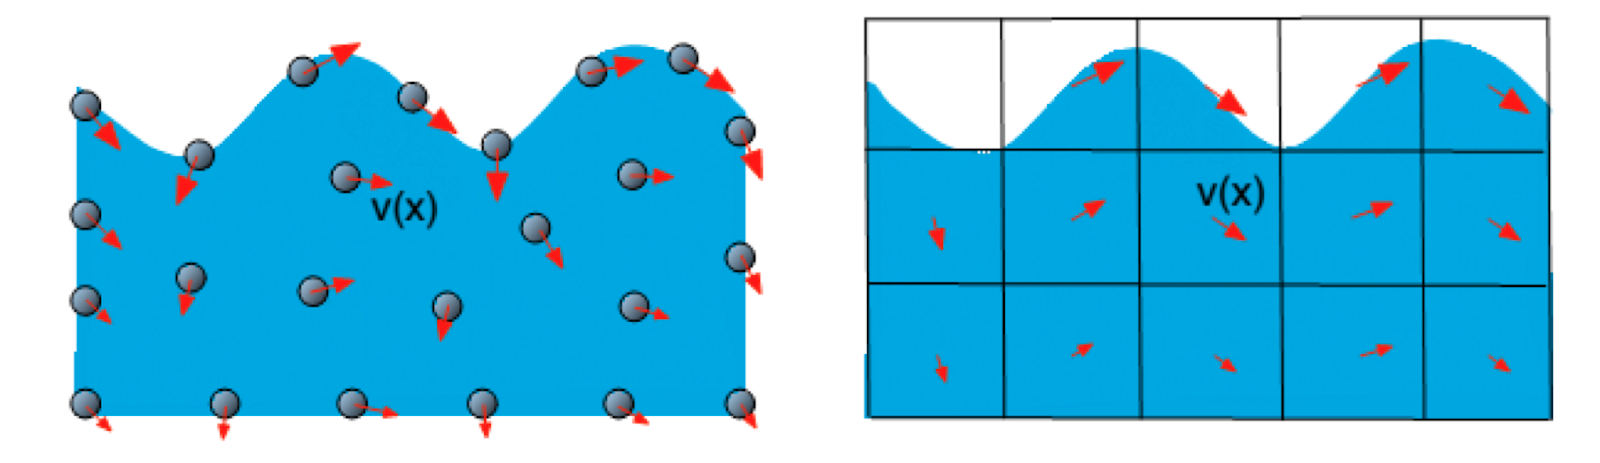
\includegraphics[scale=0.30]{sim_class}
  }
  \caption{Левый рисунок демонстрирует Лагранжево представление жидкости, жидкость представляется набором дискретных лагранжевых частиц, обладающие характеристиками необходимыми для описания траектории движения. На правом рисунке Эйлерово представление - характеристики жидкости вычисляются в фиксированных точках в пространстве, например в центре ячейки.}\label{fig:sim_class}
\end{figure}

Кроме того также выделяют смешанные методы, наиболее известным из которых является метод частиц в ячейках (PIC), разработанный в середине 50 годов Харлоу в Лос-Аламосе \cite {Harlow1963, Belocherkovsky1982, Grigoriev2000}, для моделирования плазмы. Одним из потомков PIC метода является метод сглаженных частиц (SPH - Smoothed Particle Hydrodynamics) основным отличием которого является то, что он полностью лагранжевый метод \cite{Gingold1977, Lucy1977}

Основными преимуществами метода SPH над сеточными методами являются: естественная возможность обрабатывать свободные поверхности и поверхности раздела, всплески и капли, а также взаимодействие со сложными границами и твердыми неподвижными объектами, кроме того гарантируется выполнение условия сохранение массы \cite {Müller2003, Müller2005, Keiser2005, Solenthaler2007, Solenthaler2008, Becker2007}. Изначально этот метод был предложен для решения задач, связанных с моделированием движения небесных тел, формирования звезд и галактик \cite{Gingold1977, Lucy1977}.

При моделировании методом SPH жидкость представляется набором «частиц» - дискретных элементов. Частицы характеризуются позицией в пространстве, скоростью и массой. Для представления любой физической величины  в методе SPH используется концепция интегрального представления:
\begin{equation}
\label{eq:int_rep}
A(x) = \int_{\Omega}A(x^{'})\delta (x-x^{'})dx^{'}
\end{equation}

где \(\Omega\)-некоторая область, \(dx^{'}\)-элемент объема, \(\delta (x-x^{'})\)- функция Дирака.

Если функция Дирака заменить функцией \(W\), так называемым сглаживающим ядром, с заданным радиусом сглаживания \(h\), то ~\ref{eq:int_rep} можно записать в следующем виде:
\[
A(x) = \int_{\Omega}A(x^{'})W(x-x^{'}, h)dx^{'}
\]

Сглаживающее ядро должно удовлетворять следующим условиям:
\begin{align}
\int W(x-x^{'},h)dx^{'}=1, \nonumber \\
\lim_{h\rightarrow0}W(r, h) = \delta (r). \nonumber
\end{align}

Влияние каждой частицы на свойства другой оценивается в соответствии с ее плотностью \(\rho\) и расстоянием до интересующей частицы. Математически это описывается следующим образом:
\[
A(x)=\int_{\Omega}\frac{A(x^{'})}{\rho(x^{'})}W(x-x^{'},h)dx^{'}.
\]

Заменяя интегрирование  на суммирование по соседним частицам, получаем:
\[
A(x)=\sum_{j}m_j\frac{A_j}{\rho_j}W(\left | x-x_{j} \right |,h)dx^{'}.
\]
Где \(m_j\)-масса частицы \(j\), \(A_j\) - значение величины \(A\) для частицы \(j\), \(\rho\)-плотность, связанная с частицей \(j\) и \(W\) - функция ядра. Например, плотность частицы может быть выражена как:
\[
A(x)=\sum_{j}m_j\frac{A_j}{\rho_j}W(\left | x-x_{j} \right |,h)dx^{'}=A(x)=\sum_{j}m_jW(\left | x-x_{j} \right |,h)dx^{'}.
\]
В общем случае этапы расчета смещение частицы относительно позиций на предыдущей итерации \(x(t)\), \(v(t)\) описывается следующим образом, сначала осуществляется поиск всех соседних частицы в пределах заданного радиуса сглаживания, затем рассчитываются силы, действующие на частицу, и ускорения и, наконец, вычисляется новая скорость и позиция частицы \(x(t+1)\), \(v(t+1)\).

\subsection{моделирование динамики вязкой жидкости}\label{subsec:ch1/sec4/sub1}

Модель движения несжимаемой жидкости описывается системой дифференциальных уравнений Навье-Стокса:
\begin{equation}
\label{eq:nstocs_eq1}
\rho \left ( \frac{\partial }{\partial t} + \mathbf{u} \cdot \bigtriangledown \right )\mathbf{u}=-\bigtriangledown p + \mu \bigtriangledown \cdot (\bigtriangledown \mathbf{u})+f
\end{equation}
\begin{align}
\bigtriangledown \cdot \mathbf{u} = 0 \nonumber
\end{align}
Где \(\mu\)- это коэффициент вязкости жидкости, \(f\)- сумма всех внешних сил, \(\mathbf{u}\)-скорость, \(p\)-давление. Отметить, что поскольку частицы движутся вместе с жидкостью, индивидуальная производная некоторой величины \(q\) равная полной производной \(q\frac{Dq}{Dt}=\frac{\partial q}{\partial t}\ + u \cdot \bigtriangledown q\) - это просто частная производная по времени что означает, что конвективный член в ~\ref{eq:nstocs_eq1} равен нулю \cite {Müller2003, Sedov1970}

В правой части уравнения ~\ref{eq:nstocs_eq1} описаны силы, а именно: давление \(-\bigtriangledown p\), внешние силы \(mg\) и силы вязкости \( \mu \bigtriangledown^{2}\mathbf{u} \). Уравнение движения для частицы \(i\) ~\ref{eq:nstocs_eq1} можно переписать следующим образом:
\begin{equation}
\label{eq:common_disk}
m_i\frac{D\mathbf{u}_i}{Dt}=\mathbf{F}_i^{presssure} + \mathbf{F}_i^{viscosity} + \mathbf{F}_i^{external}
\end{equation}
\begin{align}
a_i=\frac{D\mathbf{u}_i}{Dt}=\frac{F_i}{m_i} \nonumber
\end{align}
Где \(a_i\)-ускорение. Для расчета давления и сил давления используются формулы \cite {Müller2003}:
\begin{align}
p=k(\rho - \rho_0) \nonumber 
\end{align}
\begin{align}
F_{i}^{pressure}=-\sum_{j}m_j\frac{p_i+p_j}{2 \rho_j}\bigtriangledown(r_i-r_j, h) \nonumber
\end{align}
Где \(k\)– газовая постоянная Больцмана. Для расчета силы вязкости используется следующая формула \cite {Müller2003}:
\begin{align}
F_{i}^{viscosity}=-\sum_{j}m_j\frac{v_i-v_j}{2 \rho_j}\bigtriangledown^{2}(r_i-r_j, h) \nonumber
\end{align}

Для расчета плотности используется ядро \(W_{poly6}\) \cite {Müller2003}:
\[
    W_{poly6}(r,h)= \frac{315}{64\pi h^{9}}
    \begin{cases}
    (h^{2}-r^{2})^{3}, \text{если } 0 \leqslant r \leqslant  h \\
    0, \text{иначе} 
    \end{cases}
\]

Стоит отметить, что использование \(W_{poly6}\) для расчета других свойств и сил может привести к неверным результатам. Например, для вычисления давления его использование приводит к кластеризации частиц, находящихся близко друг к другу, так как градиент ядра стремится к нулю при  приближении к центру и, следовательно, отталкивающие силы исчезают \cite {Müller2003}. В работе \cite {Desbrun1996} для решения этой проблемы было предложено использовать модифицированную версию ядра \(W_{poly6}\):
\[
    W_{spiky}(r,h)= \frac{15}{\pi h^{6}}
    \begin{cases}
    (h^{2}-r^{2})^{3}, \text{если } 0 \leqslant r \leqslant  h \\
    0, \text{иначе} 
    \end{cases}
\]

Для вычисления сил вязкости ядро \(W_{poly6}\) также не подходит, так как его лапласиан почти везде отрицателен и силы, действующие между двумя близкими частицами, будут увеличивать относительную скорость частиц, что в свою очередь будет уменьшать стабильность системы \cite {Müller2003}.  Для вычисления сил вязкости используется ядро:
\[
    W_{viscosity}(r,h)= \frac{15}{2\pi h^{3}}
    \begin{cases}
    -\frac{r^{3}}{2h^{3}}+\frac{r^{2}}{h^{2}} \frac{r}{2h} - 1, \text{если } 0 \leqslant r \leqslant  h \\
    0, \text{иначе} 
    \end{cases}
\]
лапласиан, которого положителен везде.

\begin{figure}[ht]
  \centerfloat{
    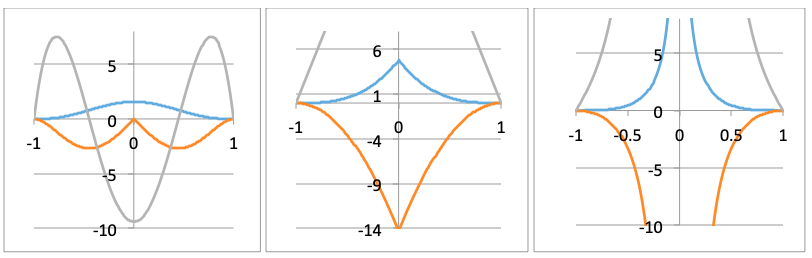
\includegraphics[scale=0.50]{ker_kind}
  }
  \caption{Сглаживающие ядра \(W_{poly6}\), \(W_{spiky}\), \(W_{viscosity}\) слева направо, представленные в работе \cite {Müller2003}. Синей линией показаны ядра, красной градиенты и зеленой лапласианы, соответственно.}\label{fig:ker_kind}
\end{figure}

Базовый алгоритм SPH не предполагает не сжимаемости моделируемой жидкости, что является одним из ключевых недостатков метода, так как подобные свойства довольно сложно воспроизвести в не сеточном методе. Однако для решения этой проблемы было предложено несколько модификаций стандартного метода SPH: WSPH \cite {Becker2007}, ISPH \cite {Shao2003, CUMMINS1999584} и PCI SPH \cite {Solenthaler2009}. Метод WSPH для обеспечения небольших колебаний плотности, при вычислении давления используется параметр жесткости \(k=c_{s}^2\) где \(c_{s}\) - скорость звука в веществе. Параметр \(k\) подобран таким образом, что скорости звука достаточно для того, чтобы сдерживать флуктуации плотности на достаточно малом уровне ~1\%  \cite {Solenthaler2009} согласно \cite {Monaghan2005}
\[
\frac{\left | \delta \rho \right |}{\rho_{0}}=\frac{\left | \boldsymbol{u} \right |^2}{c_{s}^2},
\]
где \(\boldsymbol{u}\) – максимальная скорость жидкости, \(\left | \delta \rho \right |\) и \(\rho_{0}\) плотность \(\frac{\left | \delta \rho \right |}{\rho_{0}} \sim \eta \) и, следовательно, \(k=c_{s}^{2}=\frac{\left | \delta \boldsymbol{u} \right |^{2}}{\eta}\). Однако, необходимо не  забывать о стабильности системы и выполнение критерия Куранта — Фридрихса — Леви \cite {Courant1967}
\[
\Delta t_{c} \leq \alpha \frac{h}{c}
\]
где \(h\) - радиус сглаживания, \(\alpha \sim 0.4\), \( c \)-скорость звука, как можно заметить неравенство будет выполняться только в случае достаточно маленького временного шага.

ISPH использует метод проекций, введенный в работах \cite {Temam1968, Chorin1968}: скорости на каждом шаге проектируются в бездивергентное векторное поле:
\[
\boldsymbol{div}\vec{u}=0
\]
решается уравнение Пуассона:
\begin{equation}
\label{eq:puasson}
\bigtriangledown^{2} p^{n+1}=\frac{\rho}{\Delta t}\bigtriangledown \cdot \boldsymbol{u}^{*}
\end{equation}
где \(\boldsymbol{u}^{*}\) промежуточное значение скорости, полученное из \(\boldsymbol{u}^{n}\) ( \(n\)– номер итерации ) путем подстановки \(\boldsymbol{u}^{n}\) в уравнение движения ~\ref{eq:common_disk}, игнорируя при этом градиент давления:
\[
m_i\frac{\textbf{u}_{i}^{*} -\textbf{u}_{i}^{n}}{\Delta t} = \mathbf{F}_i^{viscosity} + \mathbf{F}_i^{external},
\]
Вычислив значение давление на шаге \( n+1 \), вычисляется новое значение скорости:
\[
\textbf{u}^{n+1}=\textbf{u}^{*}+\frac{\Delta t}{\rho}\bigtriangledown p^{n+1}.
\]

Таким образом, гарантируется выполнение свойства несжимаемости на следующей итерации. Этот метод стабилен при большом временном шаге, но требует большое количество вычислений на одну итерацию.
При выборе оптимального варианта мы ориентировались как на минимизацию вычислительных затрат в единицу времени и возможность работы симуляции при относительно большом временном шаге, так и на приемлемый уровень точности получаемого решения. Всем этим требованиям отвечает метод PCI SPH (predictor-corrector incompressible smoothing particle hydrodynamics) \cite {Solenthaler2009}, в котором несжимаемость жидкости обеспечивается путем использования схемы “предиктор-корректор” для определения давления в точках пространства, занимаемых частицами. Для этого информация о флуктуациях плотности активно распространяется через жидкость и значения давления обновляются пока значения плотности во всей системе не станет удовлетворительными. При таком подходе исчезает необходимость решать уравнение Пуассона для давления ~\ref{eq:puasson} требующая значительных вычислительных затрат, и в то же время остается возможность корректной работы симуляции с большим временным шагом - более чем на порядок большем чем при использовании метода WSPH. На каждой итерации для всех частиц рассчитываются позиции и скорости \(x_{i}^{*}(t+\Delta t)\), \(v_{i}^{*}(t+\Delta t)\) исходя из \(x_{i}^{*}(t)\), \(v_{i}^{*}(t)\). Затем рассчитывается отклонение плотности:
\[
\rho_{err_{j}}^{*}(t+\Delta t)=\rho_{i}^{*}(t+\Delta t) - \rho_{0},
\]
где \(\rho_{i}^{*}(t+\Delta t) + \rho_{0}=\sum_{j} m_{j} W(x_{ij}^{*}, h) \), \(x_{ij}^{*}=x_{i}^{*}(t + \Delta t)-x_{j}^{*}(t + \Delta t)\),
которое используется для коррекции давления и, как следствие, сил давления:
\[
p_{i}(t) += \delta \rho_{err_{i}}^{*}(t+\Delta t),
\]
где \(\delta\) - рассчитано заранее значение, которое определяется по следующей формуле:
\[
\delta=\frac{-1}{\beta(-\sum_{j}\Delta W_{ij}^{0} \cdot \sum_{j}\Delta W_{ij}^{0}-\sum_{j}\Delta W_{ij}^{0} \cdot \Delta W_{ij}^{0})} ,
\]
\[
\beta=2(\frac{m_i \cdot \Delta t}{\rho_0})^2 ,
\]
\(W_{ij}^{0}=W(x_{ij}^{0})\), \(x_{ij}^{0}\) - это начальная позиция прототипной частицы. И наконец, силы давления рассчитываются следующим образом:
\[
F_{i}^{p}(t)=-m_i \sum_{j} m_j \left ( \frac{p_i(t)}{(\rho_{i}^{*})^2} + \frac{p_j(t)}{(\rho_{j}^{*})^2} \right )\Delta W(x_{ij}, h)
\]
Эта процедура повторяется пока \( max( \rho_{err_{i}}^{*} ) \) будет не больше определенного пользователем порогового значения (обычно 1\% - 3\% от характерной величины , для воды 1000 кг/м\textsuperscript{2}). Предлагается, проделывать не более трех итераций, чтобы ограничить колебание давления.

Стоит также отметить, что при смещении частиц во временные позиции список соседей, вообще говоря, может измениться. Но для повышения производительности алгоритма предполагается использовать старое множество соседей (что почти всегда выполняется; даже если есть несоответствия, то, как правило, на границе расстояния сглаживания, что дает минимальный вклад в общую величину) и только пересчитывать расстояния. Это приближение приводит к небольшим ошибкам в оценках плотности и давления, которыми можно пренебречь \cite{Solenthaler2009}. Схема алгоритма PCI SPH продемонстрирована ниже схема \ref{algo:pcisph}
\begin{algorithm}
\label{algo:pcisph}
\SetAlgoLined
\SetKwFunction{Union}{Union}\SetKwFunction{FindNeighbour}{FindNeighbour}\SetKwFunction{ComputeForce}{ComputeForce}\SetKwFunction{PredictVelocity}{PredictVelocity}\SetKwFunction{PredictPosition}{PredictPosition}\SetKwFunction{PredictDensity}{PredictDensity}\SetKwFunction{PredictDensityVariation}{PredictDensityVariation}\SetKwFunction{ComputeVelocity}{ComputeVelocity}\SetKwFunction{ComputePosition}{ComputePosition}
\SetKwInOut{Input}{input}\SetKwInOut{Output}{output}
\Input{$\mathcal P$ array of particles}

\ForEach{$p \in \mathcal P$}
{
${N_{p}} \leftarrow$ \FindNeighbour{$p, \mathcal P $}\;
}
\ForEach{$ p \in \mathcal P $}{
$F^{v,g,ext}(t) \leftarrow$ \ComputeForce{$p, \mathcal P $}\;
$p(t) \leftarrow 0.0$\;
$F^{p}(t) \leftarrow 0.0$\;
 }
 \While{$\rho_{err}^{*}(t+1)>\eta || (iter < minIterations)$}{
 \ForEach{$p \in \mathcal P$}{
    ${v_{p}^{*}(t+1)} \leftarrow$ \PredictVelocity{$p$}\;
    ${x_{p}^{*}(t+1)} \leftarrow$ \PredictPosition{$p$}\;
 }
 \ForEach{$p \in \mathcal P$}{
    $\rho_{err}^{*}(t+1) \leftarrow$ \PredictDensity{$\mathcal{P}$}\;
    $\rho_{err}^{*}(t+1) \leftarrow$ \PredictDensityVariation{$\mathcal{P}$}\;
    $p_{p}(t) += f(\rho_{err}^{*}(t+1))$\;
 }
 \ForEach{$p \in \mathcal P$}{
    $F^{p}(t) \leftarrow$ \ComputeForce{$p, \mathcal P $}\;
 }
 }
 \ForEach{$p \in \mathcal P$}{
    ${v_{p}(t+1)} \leftarrow$ \ComputeVelocity{$p$}\;
    ${x_{p}(t+1)} \leftarrow$ \ComputePosition{$p$}\;
 }
\caption{Схема алгоритма PCI SPH}
\end{algorithm}

\subsection{Неподвижные объекты и границы}\label{subsec:ch1/sec4/sub2}

Для обработки взаимодействия частиц с границей было предложено несколько методов, зачастую использующихся в различных реализациях PCI SPH:

\begin{itemize}
\item основанный на использование корректирующих сил \cite {Müller2004}
\item основанный на корректировки сил и позиций \cite {Becker2009}
\end{itemize}

Основным недостатком вышеуказанных методов является сложность обработки взаимодействия частиц с границей сложной геометрии. Одним из возможных решений данной проблемы является метод, предложенный в работе  \cite {Ihmsen2010}, основной особенностью данного подхода является использование граничных частиц. Подобная техника позволяет корректно обрабатывать контакт с границей, а кроме того, дает возможность создавать границы разных форм, не опасаясь залипания частиц. Граница представляется в виде набора граничных частиц, расположенных в узлах решетки с заданным шагом; для каждой такой частицы используются те же характеристики, что и для обычных частиц, но, в отличие от них, граничные частицы неподвижны рисунок \ref{fig:boundary}
\begin{figure}[ht]
  \centerfloat{
    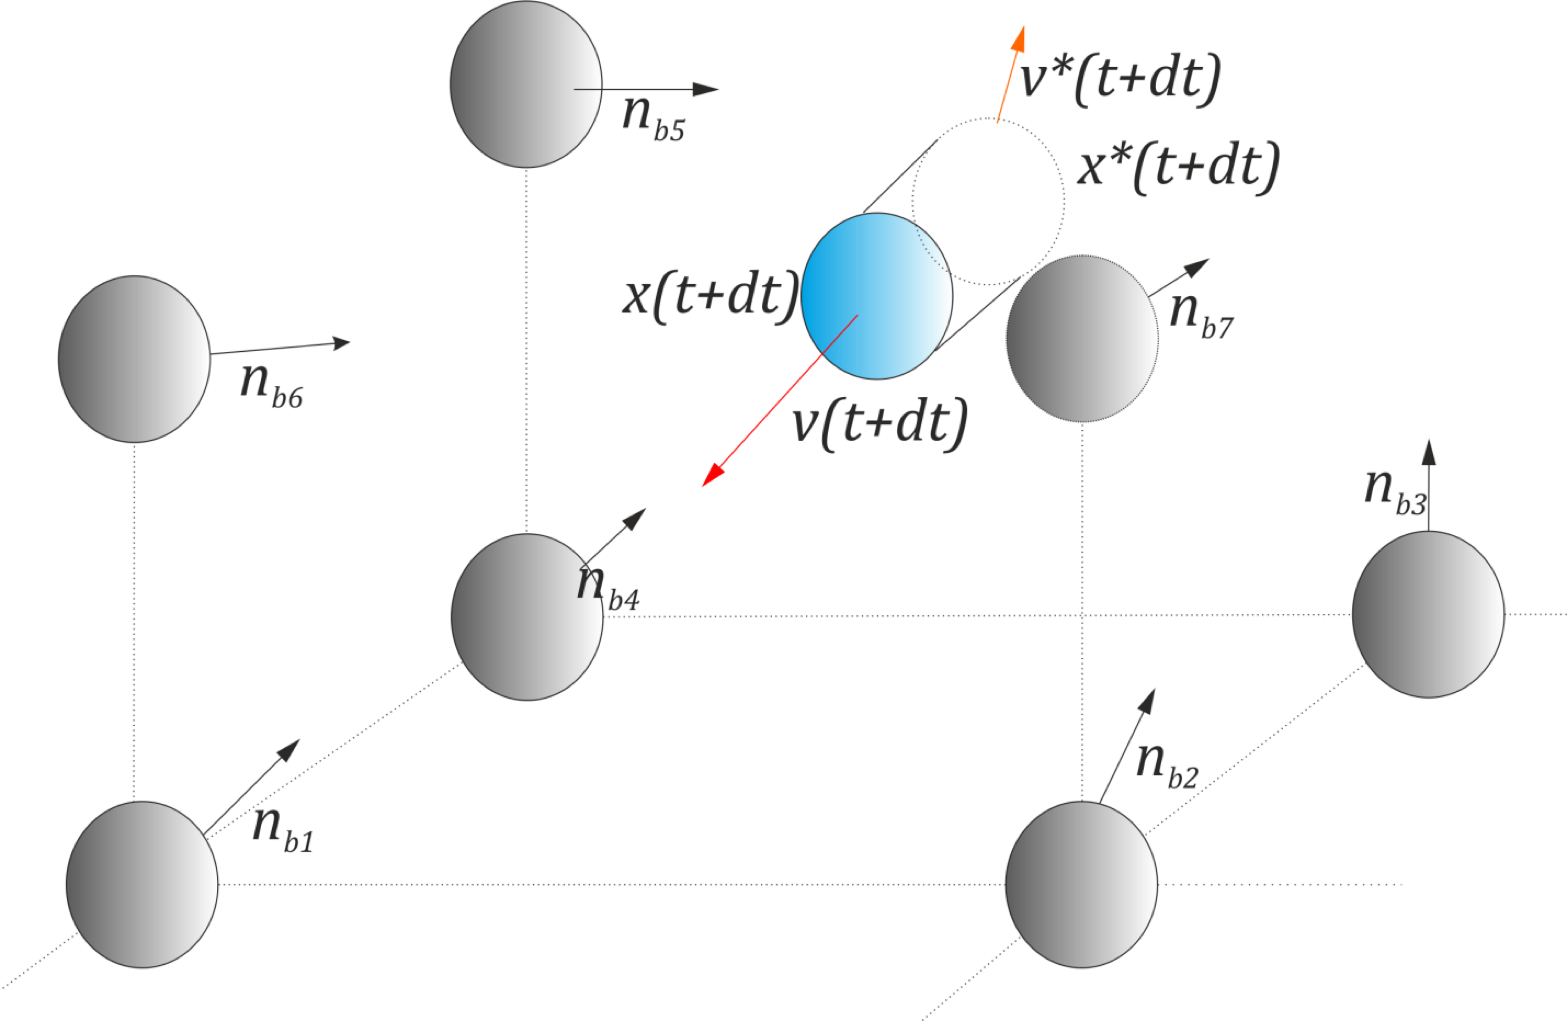
\includegraphics[scale=0.20]{boundary}
  }
  \caption{Взаимодействие граничных частиц с частицей жидкости, залетевшей в один из углов ограничивающего объема. Красной стрелкой показано направление и величина скорости \(v(t+dt)\), черными стрелками показаны нормали, исходящие из граничных частиц, представленные серыми сферами. Оранжевой стрелкой и прозрачной сферой обозначено направление скорости и положение частицы жидкости \(v^{*}(t+dt)\) и \(x^{*}(t+dt)\) после взаимодействия с границей.}
\label{fig:boundary}
\end{figure}

Взаимодействие между частицами и граничными частицами обрабатывается следующим образом, для каждой частицы, которая имеет в списке соседей граничные частицы, считаются граничные силы \(F^{boundary}\), которые влияют на распределение плотности жидкости. Отметим, однако, что частица попадает в поле действия граничных сил, только в том случае если \(\left \| x_i - x_{boundary}  \right \| \leq \frac{h}{2}=r_0\) где \(x_i\) – позиция \(i\)-й частицы \(x_{boundary}\) – позиция граничной частицы. Согласно описываемой модели, граничные частицы влияют на координаты и скорость \(i\)-й частицы следующим образом:
\[
v_{i}^{*}(t + \Delta t) = \epsilon \left [ v_{i}(t+\Delta t) \right ]_{t}
\]
где, \(\left [ v_{i}(t+\Delta t) \right ]_{t} = v_{i}(t+\Delta t) - \left [ v_{i}(t+\Delta t) \right ]_{n}\), \(\left [ v_{i}(t+\Delta t) \right ] = (v_{i}(t_i + \Delta t)\cdot n_b) \cdot n_b \) и \(n_b\) - нормаль, \( \epsilon \in \left [ 0, 1 \right ] \). При этом позиция частицы корректируется в соответствии с информацией о множество частиц граница, которые попадают окрестность:
\[
x_{i}^{*}(t+\Delta t) = x_{i}(t+\Delta t) + \frac{1}{\sum_{b}w_{ib}^{c}}\sum_{b}w_{ib}^{c}(r_0 - \left \| x_{ib} \right \|)\frac{n_{i}^{c}}{\left \| n_{i}^{c} \right \|}
\]
где \(n_{i}^{c}=\sum_{b}w_{ib}^{c}n_b\), \(n_{b}\) - нормаль к границе, направленная из граничной частицы, если граничная частица находится на пересечении нескольких граней ограничивающего объема, то нормаль из этой частицы считается как сумма нормалей этих граней, \(w_{ib}^{c}=max(0, \frac{r_0 - \left \| x_{ib}^{*} \right \|}{r_0})\), \(\left \| x_{ib} \right \| = \left \| x_{i}(t+\Delta t) - x_{b} \right \|\).
